% This is samplepaper.tex, a sample chapter demonstrating the
% LLNCS macro package for Springer Computer Science proceedings;
% Version 2.20 of 2017/10/04
%
\documentclass[runningheads]{llncs}
%
\usepackage{graphicx}
% Used for displaying a sample figure. If possible, figure files should
% be included in EPS format.
%
% If you use the hyperref package, please uncomment the following line
% to display URLs in blue roman font according to Springer's eBook style:
% \renewcommand\UrlFont{\color{blue}\rmfamily}

\begin{document}
%
\title{A Geovisual Framework for Data Exploration in Government Open Data Using NIBRS (National Incident-based Reporting System) for Law Enforcement Agencies}
%
%\titlerunning{Abbreviated paper title}
% If the paper title is too long for the running head, you can set
% an abbreviated paper title here
%
\author{Michael Crowder\inst{1}\and
Lauren Darr\inst{1}\and
Gerardo Garza\inst{1}\and
Brent Allen\inst{1}}
%
%\authorrunning{F. Author et al.}
% First names are abbreviated in the running head.
% If there are more than two authors, 'et al.' is used.
%
\institute{Southern Methodist University Master of Science Data Science Program \and
Dallas, Texas, United States of America}
%
\maketitle              % typeset the header of the contribution
%
\begin{abstract}
In this paper we present a geovisual framework for data exploration in government open data using NIBRS (National Incident Based Reporting System) for users that are considered novice data users. The open data movement is relatively new, and the average citizen is not proficient in data exploration methods, understanding and execution. We present the reader with a brief history and definition of open data in the government segment, specifically with law enforcement agencies. The paper then presents a geovisual framework for novice users that can be implemented by local government agencies when the 2021 NIBRS standard goes into effect for all 18,000 law enforcement agencies around the United States with the use of the City of Dallas Police Open Data Police Incidents data. We hope to conclude a general framework for geo-visualizations for law enforcement agencies to educate the public of the work and services provided to them.

\keywords{First keyword  \and Second keyword \and Another keyword.}
\end{abstract}
%
%
%
\section{Introduction}
The open data movement unsurprisingly came on the heels of internet globalization and is still developing rapidly [1]. In 2007 prominent academics and open data champions met to outline the guiding principles of open public data [2]. In 2013, the United States government formally recognized open public data as a valuable national resource in a memorandum to the heads of executive departments and agencies titled “M-13-13 Open Data Policy-Managing Information as an Asset” [3]. The motivation behind the memo was to make information resources accessible, discoverable and usable by the public [3]. As one of the key pillars defined in the memo, accessibility suggests that open data must be made available in convenient, modifiable and open formats. These formats must be machine-readable and should be made available to the widest range of users for the widest range of purposes [3]. The larger goal of open data is to promote transparency in democratic governments, citizen participation, and drive innovation that can ultimately generate economic value [4]. 

A majority of the population does not actively execute data exploration methods in their daily life. Another barrier to understanding is the need for more education in the realm of data and statistics so that citizens can evaluate and make judgements about the validity of claims [8]. These two potential issues leave us with a problem that this paper tries to solve at least in terms of the geovisual aspect of data exploration by a novice user.

For open data in government to provide transparency as intended there is a need for resources from two contributing parties. First, there is a need for information or data from a government agency. This project focuses on data generated by the National Incident-Based Reporting System (NIBRS) set forth by the Federal Bureau of Investigation (FBI) Uniform Crime Reporting (UCR) Program in partnership with the Bureau of Justice Statistics (BJS) in 1989 [5]. The NIBRS program succeeded the Summary Reporting System (SRS) which provided aggregate statistics from law enforcement agencies with only one crime recorded per-incident regardless of the number of crimes that occurred [5]. NIBRS provides uncombined incident information that is more easily usable by interested parties [6]. However, NIBRS has been slowly adopted by law enforcement agencies on a voluntary basis until now [5]. Recently, the FBI set forth a NIBRS compliancy deadline of 2021 for all law enforcement agencies in the U.S. Former FBI director, James Comey, emphasized the importance of conforming to NIBRS in a 2015 speech to the International Association of Chiefs of Police (IACP): “NIBRS is a way in which we can collect data that will identify patterns, trends, and help us prevent crime and have thoughtful, informed conversations at the national level” [7]. The thoughtful conversations NIBRS will surely generate is still subject to the second necessity for true transparency: statistical literacy of the data consumers. 

In this paper a ‘novice user’ is defined as an individual working within, or contracted by, a law enforcement agency that does not necessarily have an extensive education or background experience in data handling, statistics, or data visualization. There are approximately 18,000 U.S. law enforcement agencies across federal, state, county, and local jurisdictions in the U.S. [9]. These agencies can range in department size from 1-30,000 officers with the majority of agencies having 10 or fewer officers [9]. This wide range in officer employment suggests that the number of civilians employed by U.S. law enforcement agencies also ranges widely. It is safe to assume that the majority of law enforcement agencies, particularly at the local level, are without funding for advanced private software, let alone a trained data analyst on staff. Furthermore, the fragmented nature of U.S. law enforcement as a collective of independent agencies means that the adoption of data handling practices will also be disparate. 

In 2015, the Police Data Initiative (PDI) was launched per recommendation of President Obama’s Task Force on 21st Century Policing [10]. The PDI is a collective network of law enforcement agencies, researchers, and technologists already developing and delivering best practices for collecting and publishing public datasets as well as utilizing data and technology for the improvement of policing and community relations [10]. As of March, 2018, there are 130 contributing agencies and over 330 available data sets through the PDI website [11]. The PDI demonstrates and embraces the diversity of law enforcement agencies’ needs and resources with both large and small (**find smallest dep) department participants.

It is unsurprising that news media coverage of crime data analytics has a tendency to focus on the most ground breaking and intriguing innovations of the moment. A 2016 Science Magazine article detailed the use of advanced predictive software by agencies looking both to predict where crimes will happen and the actual individuals who may commit or become victims of crimes [11]. For example, PredPol is proprietary software that uses algorithms to predict where crimes are likely to happen during a shift [11]. While forecasting crimes is a highly pertinent application of incident data, it is not a cure-all for understanding and effectively using crime data. 

This project focuses on the potential needs of small law enforcement agencies with limited funding for technology advancement or agencies that just want to get their feet wet with NIBRS data exploration from a geospatial perspective. The goal of this project is to develop an application that can take any NIBRS data set and output a series of geospatial visualizations for exploring incident data. 

\subsection{Background and Related Work}
Richard Hamming in 1962 stated that “The purpose of computing is insight, not numbers”. Visualization in scientific computing as it’s currently known started out of a paper sponsored by the National Science Foundation. The paper acknowledged the potential gain in productivity and breakthroughs in the American scientific and engineering communities [12]. Since 1990, the Institute of Electrical and Electronics Engineers (IEEE) have held a reoccurring conference on visualization in scientific computing. The main goal of visualization is to see the unseen by interpreting the data fed into a computer. Very much of modern data visualization is comparable to the approach of abductive discovery as discussed by Charles S. Peirce (1839 – 1914). Peirce saw the scientific method as three phases: abduction, which involves making hypotheses, deduction, which infers what the state should be in the hypotheses is the case and finally induction, or the testing of the hypothesis [13].

Some of the challenges of modern visualization as it relates to sheer size of data sets is presented by Wang include, visual noise, in which we see data that are too related to each other. The second is information loss, in which data is removed because of potential errors. Thirdly, large image perception is tough on our limited aspect ratios of the device in which a user is using. Lastly high-performance requirements that are required to sometimes run large sets of data within a visualization [14].

Maps have been in use for thousands of years, maps with data have been in use for almost as long. With the rapid rise of new data sources comes the challenge of how we extract useful information. Do authors of visualizations use the original data set or combine other datasets linked by say zip codes, or census tracks to make them more useful to the novice user? [15]. The classic definition of a map is that of a plot of land scaled down on a flat medium that represents part of the Earth’s surface. The rise of information technology and scientific computing have changed map making. This rise in information has given rise to geographic information systems (GIS). A typical GIS software will have the ability to layer information on top of a map in order to tell a story with a dynamic map that a user can explore. 

There are many software types that exist for geospatial analysis. There are large commercial GIS packages like ArcView, ArcGis and ERSI, from an open source perspective there are many tools like R and Python that have many APIs that enable a user to create fairly robust geospatial visualizations with APIs like Ploty, Leaflet and GeoPandas.

From a criminal analyst’s perspective, the International Association of Crime Analysts (IACA) Standards, Methods and Technology Committee has a white paper called “Identifying High Crime Areas”. One of the first points of the white paper is that crime is seldom randomly or evenly distributed across space. The identification of high crime areas plays a key role in how law enforcement agencies operate and address crime in certain areas [16]. The paper goes through various geospatial visualizations that may be useful for the criminal analysts to ascertain high crime areas in a city.

Research on novice users in regard to data visualization is very limited. One of the few papers that do exist from Lee et. al. “How do People Make Sense of Unfamiliar Visualizations? A Grounded Model of Novice Information Visualization Sensemaking” the authors found five cognitive activities that were most common between the study participants [17]. The authors defined these five activities as the NOvice's information Visualization Sensemaking (NOVIS) model: encountering visualization, constructing a frame, exploring visualization, questioning the frame, and floundering on visualization. 

When encountering visualization, the user looks at the information visualization as a whole. Secondly the subject would construct a frame to make sense of a visualization though the reliance on items such as an axis, legend or data labels. From here the user is exploring visualization through the constructed frame. They retrieve information, recall domain knowledge and wonder around the visualization. After exploring the visualization, the user then questions the frame and attempts validation. Finally, failing in any of the above steps takes us to floundering on visualization leading to frustration and confusion.

\section{Data}
\subsection{Data Source}
Data was sourced from the Dallas Open Data website[cite]. This website is provided by the city via the hosting software service Socrata. This website is designed to provide transparency to citizens and developers with a variety of data sets that pertain to city governance, services, and culture. The NIBRS based data set of interest on Dallas Open Data is titled Police Incidents. The Police Incidents data set is updated daily and includes incident reports dating back to June 1, 2014.

As of April, 2018, there are approximately 352,000 incident entries and there are 103 incident attributes. The complete list of incident attributes is found in the appendix (cite). Some important features of an individual incident report include the unique identifier, ‘Incident Number w/Year’, the location details of the incident, the descriptive details of the complainant, the reporting officer details, and the details of the type of incident that occurred.

\subsection{Accessing Data}
The Police Incidents data set was accessed using the Socrata application programming interface (API) and R (version) programming language within the R-Studio (version) programming environment. 

**Include more information about how the API works, the documentation from Socrata and how the R Socrata library was used to access the data and store it into a df. Every time the code is run the df is updated with whatever new entries have been added to the data set.

\subsection{Data Pre-Processing}
Data pre-processing, or data cleansing, is the important step of determining what kind and how many inaccuracies are present in a data set. It is safe to assume that most data sets have inaccuracies. Examples of potential problems a data set may include: missing values, incorrect attribute data types, misspellings, incorrectly entered data, duplicate entries, and more (CITE some info about data cleaning process).
Since this is written with a novice user in mind, should we include actual examples of code to detail the process of data cleaning. 

\section{Methods}
\subsection{Incident type: Burglary}
There is a wide variety of incident types recorded every day by police departments everywhere. In order to effectively visually explore crime incidents, it is important to focus in on specific types of incidents. 

\subsection{Burglary mapped by zip code}
Why it is important to map by zip code.
Why zip code helps with understanding spatial pattern.

\subsection{Burglary mapped by zip code and year}
Can we visually see a difference in the pattern of burglary around Dallas from year to year? 
What are the pitfalls?
If there appear to be trends from year to year what could be done next to hone in on pattern changes? (bar graph?)

\section{Ethical Considerations}
The dataset we use in this paper contains the names and addresses of complainants of the burglaries displayed in this research. We did not map out the addresses of the complainants of the burglaries, there was no reason to do so. The practice of including the name and address of the complainant is actually very common in public safety open datasets. Unwarranted publication of personal addresses could pose a threat to those that report crimes. There also inlies the possibility of businesses scraping the data of complainants to target advertisements and products in what could be a sensitive time for the complainant. 

The “Incident Address” in our data is the address where an incident occurred. There exist many possible ways in which data can be displayed on maps. Heat maps present opportunities to adjust density in order to magnify the visualization of incident location. This could cause the potential for an area to appear to have more activity than it actually does. If a user of the geovisual tool is looking at say crime in an area they are considering purchasing a house, or a user is looking for a place to place a business the density on the heat map could turn that user away from an otherwise safe area.

Those preparing geovisualization for novice users should take into account potential considerations on how the visualization could affect an individual party, or a community as a whole. A famous case of geovisualization in journalism occurred in 2012 just months after the Sandy Hook Elementary shooting. The publication published three online maps that contained a two-county area with the names and addresses of those that were permit holders. 

Some ground-rules, or guidelines to consider when preparing a geovisualization for novice users would be to research data journalism guidelines. Craig, Ketterer, and Yousuf, in their paper “To Post or Not to Post: Online Discussion of Gun Permit Mapping and the Development of Ethical Standards in Data Journalism provides some recommended frames when considering publishing information that could raise ethical questions. The first is freedom verus responsibility and journalistic purpose, which purposes that data should not be posted only because its already in a public dataset. The second frame is privacy and verification, to attempt to measure the risks to a person’s private life. Thirdly are consequences to the individual if the information is wrong. Finally, what alternatives are available, such as showing trends or joining with other data to tell the same story [18].


\section{Conclusion}

\subsubsection{Acknowledgments}

%
% ---- Bibliography ----
% Bibliography has not been updated as of 4/25/18 
% Must fix use of footnotes and references before implement (LD)
% BibTeX users should specify bibliography style 'splncs04'.
% References will then be sorted and formatted in the correct style.
%
% \bibliographystyle{splncs04}
% \bibliography{mybibliography}
%
\begin{thebibliography}{8}
\bibitem{ref_article1}
Author, F.: Article title. Journal \textbf{2}(5), 99--110 (2016)

\bibitem{ref_lncs1}
Author, F., Author, S.: Title of a proceedings paper. In: Editor,
F., Editor, S. (eds.) CONFERENCE 2016, LNCS, vol. 9999, pp. 1--13.
Springer, Heidelberg (2016). \doi{10.10007/1234567890}

\bibitem{ref_book1}
Author, F., Author, S., Author, T.: Book title. 2nd edn. Publisher,
Location (1999)

\bibitem{ref_proc1}
Author, A.-B.: Contribution title. In: 9th International Proceedings
on Proceedings, pp. 1--2. Publisher, Location (2010)

\bibitem{ref_url1}
LNCS Homepage, \url{http://www.springer.com/lncs}. Last accessed 4
Oct 2017
\end{thebibliography}


%%%%All code below is not part of the capstone paper, it will serve as examples for formatting and then removed.%%%%


\subsubsection{Sample Heading (Third Level)} Only two levels of
headings should be numbered. Lower level headings remain unnumbered;
they are formatted as run-in headings.

\paragraph{Sample Heading (Fourth Level)}
The contribution should contain no more than four levels of
headings. Table~\ref{tab1} gives a summary of all heading levels.

\begin{table}
\caption{Table captions should be placed above the
tables.}\label{tab1}
\begin{tabular}{|l|l|l|}
\hline
Heading level &  Example & Font size and style\\
\hline
Title (centered) &  {\Large\bfseries Lecture Notes} & 14 point, bold\\
1st-level heading &  {\large\bfseries 1 Introduction} & 12 point, bold\\
2nd-level heading & {\bfseries 2.1 Printing Area} & 10 point, bold\\
3rd-level heading & {\bfseries Run-in Heading in Bold.} Text follows & 10 point, bold\\
4th-level heading & {\itshape Lowest Level Heading.} Text follows & 10 point, italic\\
\hline
\end{tabular}
\end{table}


\noindent Displayed equations are centered and set on a separate
line.
\begin{equation}
x + y = z
\end{equation}
Please try to avoid rasterized images for line-art diagrams and
schemas. Whenever possible, use vector graphics instead (see
Fig.~\ref{fig1}).

\begin{figure}
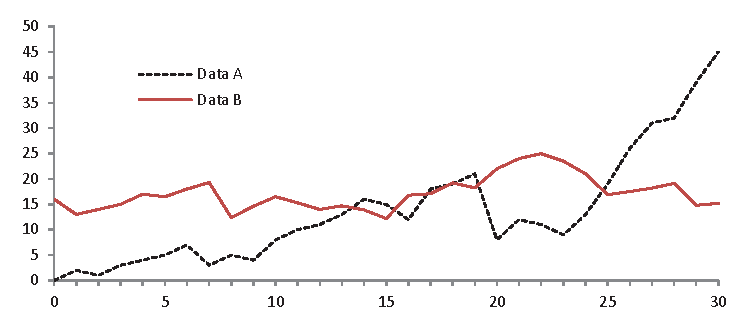
\includegraphics[width=\textwidth]{fig1.eps}
\caption{A figure caption is always placed below the illustration.
Please note that short captions are centered, while long ones are
justified by the macro package automatically.} \label{fig1}
\end{figure}

\begin{theorem}
This is a sample theorem. The run-in heading is set in bold, while
the following text appears in italics. Definitions, lemmas,
propositions, and corollaries are styled the same way.
\end{theorem}
%
% the environments 'definition', 'lemma', 'proposition', 'corollary',
% 'remark', and 'example' are defined in the LLNCS documentclass as well.
%
\begin{proof}
Proofs, examples, and remarks have the initial word in italics,
while the following text appears in normal font.
\end{proof}
For citations of references, we prefer the use of square brackets
and consecutive numbers. Citations using labels or the author/year
convention are also acceptable. The following bibliography provides
a sample reference list with entries for journal
articles~\cite{ref_article1}, an LNCS chapter~\cite{ref_lncs1}, a
book~\cite{ref_book1}, proceedings without editors~\cite{ref_proc1},
and a homepage~\cite{ref_url1}. Multiple citations are grouped
\cite{ref_article1,ref_lncs1,ref_book1},
\cite{ref_article1,ref_book1,ref_proc1,ref_url1}.
\end{document}
